\documentclass{beamer}
\usetheme{Madrid}
\usecolortheme{dolphin}
\usepackage{graphicx}
\usepackage{amsmath}
\usepackage{hyperref}
\usepackage{listings}
\usepackage{tikz}
\usetikzlibrary{shapes, arrows, positioning}

% Custom colors
\definecolor{aiblue}{RGB}{0, 102, 204}
\definecolor{aiyellow}{RGB}{255, 204, 0}
\definecolor{aigreen}{RGB}{0, 153, 51}

% Title page customization
\setbeamercolor{title}{fg=aiblue}
\setbeamercolor{frametitle}{fg=aiblue}
\setbeamercolor{structure}{fg=aiblue}

% Consistent font size and spacing
\setlength{\itemsep}{6pt}
\setlength{\parskip}{4pt}
\setbeamertemplate{itemize items}[circle]

\title{Adaptive Interview Simulation and Feedback using Agentic AI}
\author{Ranjit N\\ CB.SC.I5DAS21050}
\institute{[Amrita Vishwa Vidyapeetham]}
\date{\today}

\begin{document}

% Slide 1: Title Slide
\begin{frame}
    \titlepage
\end{frame}

% Slide 2: Problem Statement and Solution
\begin{frame}{Problem Statement \& Solution}
    \begin{columns}[T,onlytextwidth]
        \column{0.5\textwidth}
        \textbf{Problem Statement:}
        \begin{itemize}
            \item Ineffective and non-personalized interview preparation
            \item Lack of skill gap identification and feedback
            \item Limited access to realistic mock interviews
            \item Difficulty simulating real interview conditions
        \end{itemize}
        
        \column{0.5\textwidth}
        \textbf{Solution:}
        \begin{itemize}
            \item Multi-agent AI system for personalized practice
            \item Real-time feedback with adaptive questioning
            \item Skill gap identification and resource recommendations
            \item Comprehensive performance tracking
        \end{itemize}
    \end{columns}
\end{frame}

% Slide 3: Project Goals and Architecture
\begin{frame}{Project Goals \& Architecture}
    \textbf{Primary Goals:}
    \begin{itemize}
        \item Create a comprehensive interview preparation system
        \item Provide adaptive interview experiences
        \item Generate actionable feedback and improvement tips
        \item Ensure a seamless, intuitive local-first experience
    \end{itemize}
    
    \vspace{0.5cm}
    \centering
    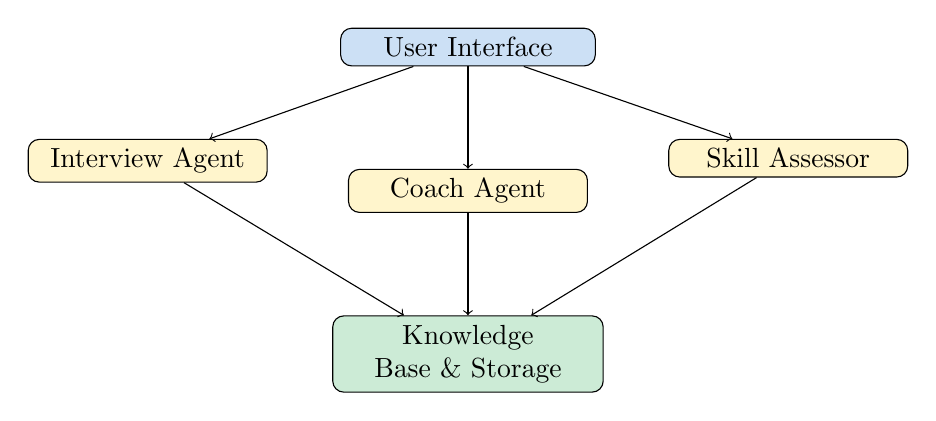
\begin{tikzpicture}[node distance=1.3cm, every node/.style={align=center}]
        \node[draw, rounded corners, fill=aiblue!20, text width=3cm] (ui) {User Interface};
        \node[draw, rounded corners, fill=aiyellow!20, text width=2.8cm, below left=of ui] (ia) {Interview Agent};
        \node[draw, rounded corners, fill=aiyellow!20, text width=2.8cm, below=of ui] (ca) {Coach Agent};
        \node[draw, rounded corners, fill=aiyellow!20, text width=2.8cm, below right=of ui] (sa) {Skill Assessor};
        \node[draw, rounded corners, fill=aigreen!20, text width=3.2cm, below=of ca] (db) {Knowledge Base \& Storage};
        
        \draw[->] (ui) -- (ia);
        \draw[->] (ui) -- (ca);
        \draw[->] (ui) -- (sa);
        \draw[->] (ia) -- (db);
        \draw[->] (ca) -- (db);
        \draw[->] (sa) -- (db);
    \end{tikzpicture}
\end{frame}

% Slide 4: Core Agents System
\begin{frame}{Core Agents System}
\small
\textbf{Interview Agent:}
\begin{itemize}
    \item Adaptive interviews with dynamic questioning
    \item Multiple interview styles (formal, casual, technical)
    \item Follow-up questions for vague responses
\end{itemize}

\vspace{6pt}

\textbf{Interview Coach Agent:}
\begin{itemize}
    \item Real-time feedback on responses
    \item STAR format analysis (Situation, Task, Action, Result)
    \item Identifies content and delivery weaknesses
\end{itemize}

\vspace{6pt}

\textbf{Skill Assessor Agent:}
\begin{itemize}
    \item Identifies skill gaps from multiple responses
    \item Maps skills to job requirements
    \item Suggests personalized learning resources
\end{itemize}
\end{frame}

% Slide 5: Enhanced AI Tools Integration
\begin{frame}{Enhanced AI Tools Integration}
    \begin{columns}[T,onlytextwidth]
        \column{0.33\textwidth}
        \textbf{Web Search API}
        \begin{itemize}
            \item Uses Serper.dev
            \item Finds tailored learning resources
            \item Ranks articles by relevance
        \end{itemize}
        
        \column{0.33\textwidth}
        \textbf{Coding Sandbox}
        \begin{itemize}
            \item Secure Python execution environment
            \item Automated test case evaluation
            \item Performance metrics
        \end{itemize}
        
        \column{0.33\textwidth}
        \textbf{RAG System}
        \begin{itemize}
            \item Local FAISS vector database
            \item Embeddings with all-MiniLM-L6-v2
            \item Contextual information retrieval
        \end{itemize}
    \end{columns}
\end{frame}

% Slide 6: Data Storage & Processing
\begin{frame}{Data Storage \& Processing}
\scriptsize
\textbf{Storage Infrastructure:}
\begin{itemize}
    \item SQLite for structured data (user profiles, sessions)
    \item FAISS for vector embeddings
    \item Local file system for transcript storage
\end{itemize}

\vspace{4pt}

\textbf{Key Functionality:}
\begin{itemize}
    \item Complete transcript persistence
    \item Vector embeddings for semantic search
    \item Export options (text, JSON with metadata)
\end{itemize}

\vspace{4pt}

\textbf{Speech Processing:}
\begin{itemize}
    \item Browser Web Speech API for speech recognition
    \item Kokoro TTS for natural-sounding TTS
    \item Local processing for privacy
\end{itemize}
\end{frame}

% Alternative layout for Slide 7
\begin{frame}{Frontend Experience}
    \begin{columns}[T]
        \column{0.48\textwidth}
        \begin{figure}
            \includegraphics[width=\textwidth]{frontend1.png}
            \caption{Starting page}
        \end{figure}
        
        \column{0.48\textwidth}
        \begin{figure}
            \includegraphics[width=\textwidth]{frontend2.png}
            \caption{Feeding context}
        \end{figure}
    \end{columns}
\end{frame}

% Slide 8: Continuing
\begin{frame}{More frontend interface}
    \begin{columns}[T]
        \column{0.48\textwidth}
        \begin{figure}
            \includegraphics[width=\textwidth]{frontend3.png}
            \caption{Main interview interface}
        \end{figure}
        
        \column{0.48\textwidth}
        \begin{figure}
            \includegraphics[width=\textwidth]{frontend4.png}
            \caption{Feedback dashboard}
        \end{figure}
    \end{columns}
\end{frame}

% Slide 9: Future Work
\begin{frame}{Future Work}
    \textbf{Planned Enhancements:}  
    \begin{itemize}
        \item Integrate the AI tools like web search, coding sandbox etc...
        \item Update the frontend to match the backend features  
        \item FAISS retrieval implementation 
        \item Transcript generation and download for future use 
        \item Add the option to upload past transcripts to use as context
    \end{itemize}
\end{frame}

% Slide 10: LLM Configuration
\begin{frame}{LLM Configuration}
    \textbf{Parameter Settings for Gemma 3:}
    \begin{itemize}
        \item \textbf{Temperature}: 0.7 for Interviewer (creativity), 0.2 for Coach/Skill Assessor (precision)
        \item \textbf{Top-p}: 0.9 to ensure controlled randomness
        \item \textbf{Max tokens}: Variable limits based on expected response length
        \item \textbf{Presence penalty}: 0.6 to reduce repetition
    \end{itemize}
    
    \textbf{Memory Management:}
    \begin{itemize}
        \item Sliding window memory for Interviewer Agent
        \item Summary memory for Coach Agent
        \item Cumulative memory for Skill Assessor
    \end{itemize}
\end{frame}

% Slide 11: Database Implementation
\begin{frame}{Database Implementation}
    \textbf{SQLite Schema Design:}
    \begin{columns}[T,onlytextwidth]
        \column{0.5\textwidth}
        \begin{itemize}
            \item \textbf{Sessions Table}\\
            Primary session metadata
            \item \textbf{Questions Table}\\
            Questions with types and sequence
            \item \textbf{Responses Table}\\
            User answers with duration
        \end{itemize}
        
        \column{0.5\textwidth}
        \begin{itemize}
            \item \textbf{Feedback Table}\\
            Structure, clarity, and relevance scores
            \item \textbf{Skills Table}\\
            Categorized skill taxonomy
            \item \textbf{SkillDemonstrations Table}\\
            Response-to-skill mapping
        \end{itemize}
    \end{columns}
    
    \vspace{0.3cm}
    \textbf{Key Features:} Foreign key constraints, indexed columns, referential integrity
\end{frame}

% Slide 12: Interviewer Agent Details
\begin{frame}{Interviewer Agent Details}
    \textbf{Question Generation Pipeline:}
    \begin{itemize}
        \item Context preparation from resume and job descriptions
        \item Dynamic and static question selection algorithm
        \item Question adaptation based on previous responses
        \item Follow-up question identification logic
    \end{itemize}
    
    \textbf{State Management:}
    \begin{itemize}
        \item Introduction → Skill assessment → Behavioral assessment → Technical validation → Wrap-up
        \item State transitions based on response quality and coverage
        \item Guard conditions to ensure interview progression
    \end{itemize}
\end{frame}

% Slide 13: Coach Agent Details
\begin{frame}{Coach Agent Details}
    \textbf{Evaluation Framework:}
    \begin{itemize}
        \item STAR Analysis: Balance of Situation, Task, Action, Result
        \item Grammar and structure evaluation
        \item Relevance detection to question intent
        \item 1-5 scale quantitative scoring system
    \end{itemize}
    
    \textbf{Feedback Generation:}
    \begin{itemize}
        \item Critical area prioritization algorithm
        \item Constructive criticism balancing
        \item Adaptive feedback based on user progress
        \item Industry-specific evaluation criteria
    \end{itemize}
\end{frame}

% Slide 14: Event-Driven Communication
\begin{frame}{Event-Driven Communication System}
    \textbf{Core Components:}
    \begin{itemize}
        \item Event Message Structure: Type, Payload, Metadata
        \item Subscription Registry: Observer Pattern Implementation
        \item Message Processing Guarantees: In-Memory Queue, Error Handling
    \end{itemize}
    
    \textbf{Benefits:}
    \begin{itemize}
        \item Decoupled Components
        \item Reactive Architecture
        \item Enhanced Maintainability
        \item Simplified Component Extension
    \end{itemize}
\end{frame}

% Slide 15: References
\begin{frame}{References}
    \scriptsize % Slightly larger text size for better readability
    \begin{thebibliography}{9}
    
        \bibitem{rag}
        Lewis, P., Perez, E., Piktus, A., Petroni, F., Karpukhin, V., Goyal, N., Küttler, H., Lewis, M., Yih, W., Rocktäschel, T., Riedel, S., \& Kiela, D. (2020).  
        \newblock Retrieval-Augmented Generation for Knowledge-Intensive NLP Tasks.  
        \newblock \textit{NeurIPS}, 9459-9468.  

        \bibitem{faiss}
        Johnson, J., Douze, M., \& Jégou, H. (2019).  
        \newblock Billion-scale similarity search with GPUs.  
        \newblock \textit{IEEE Transactions on Big Data}, 7(4), 700-708.  

        \bibitem{cot}
        Wei, J., Wang, X., Schuurmans, D., Bosma, M., Ichter, B., Xia, F., Chi, E., Le, Q., \& Zhou, D. (2022).  
        \newblock Chain of Thought Prompting Elicits Reasoning in Large Language Models.  
        \newblock \textit{NeurIPS}, 35, 24824-24837.  

        \bibitem{dialogue}
        Yao, S., Li, B., Chen, M., Zhao, L., Pan, H., Lin, X. V., et al. (2024).  
        \newblock Planning with Language Models for Dialogue Agents.  
        \newblock \textit{Proceedings of the 62nd Annual Meeting of the Association for Computational Linguistics (ACL)}, 2024.  

        \bibitem{agents}
        Park, J., O'Brien, J., Suresh, S., Zhang, A., Donahue, C., Saunders, W., \& Newton, C. (2024).  
        \newblock Generative Agents: Interactive Simulacra of Human Behavior.  
        \newblock \textit{Proceedings of the 2024 CHI Conference on Human Factors in Computing Systems (CHI)}.  

    \end{thebibliography}
\end{frame}


\end{document}
